\chapter{Alternative Technique Design}

\quad\quad 上一章中我们分析了 Apple Watch 上的交互方式,
除了语音交互外,这些方式都要求用户使用双手来完成整个交互。但实际场景中,如果用户双手空闲,
则用户完全可以使用手机完成需要完成的事情,况且在屏幕适中的手机上完成交互也只需一直手。
因此,这种交互模式从本质上就是一种不利于增加用户粘性的交互方式。
考虑使用手表时的抬碗姿势,最自然的交互自然就是在抬碗时仅用一只手便能完成全部的交互行为。

\section{Interaction Pattern}

\subsection{Tap and View Switch}

点按与视图切换的操作一共涉及五个操作:普通点按、Force Touch 点按、切换到左视图、切换到右视图、切换到上一视图。

单手手指的点击由两个两个手指的捏合操作来完成,拇指和其他四个手指的组合恰好能完成全部的点按交互,
拇指和食指的点按来替代普通点击事件,拇指和中指、无名指的捏合实现视图的切换,拇指和小指的捏合则实现返回上级视图的功能。

此外,拇指和食指的点按还能对 Force Touch 进行仿真,方法详见\ref{sub:force-touch-simu}一节。

\subsection{Swipe and Slider Control}

滑动与连续调节其实是由 Digital Crown 这一种交互手段在两种不同场景下表达,
在一般视图下滑动时能够对视图内容进行纵向调节,而当交互目标选择为滑动器(Slider Bar)时,能够对其值进行连续调整。

我们可以在单手上利用双指的相对滑动来实现这一交互。它是指由拇指在食指上的滑动,
在视图内通过上下快速滑动来实现交互对象的选取,通过闭合时的的慢速滑动来调节纵向的内容展示,
如果选取的交互对象是滑杆,那么这种滑动还能够调节滑动器的值。

\subsection{Force Touch Simulation}
\label{sub:force-touch-simu}

一项开源项目 Forcify \cite{Huxpro:2016ua} 是一个针对 Web 端触摸事件的通用框架,
将任何 Web 应用里的点击事件作为 3D Touch
\footnote{Apple 对 Force Touch 技术在 iOS 设备上重新命名。}
进行处理,对不具备 Force Touch 功能设备采用触摸事件延时处理的方法进行模拟。
然而,其处理事件的延时时间需要开发者自行定义,且触发 Force Touch 的力度是线性函数。
为此,我们应对这个方法进行改进。

首先,对屏幕上的触摸事件划分为两个阶段,第一个阶段的触摸事件处理为普通触摸的触摸事件,
第二个阶段的触摸事件处理为 Force Touch,并使用 DELAY 表示触发 Force Touch 的时间延时,
DURATION 表示 Force Touch 从最小值到最大值的持续时间。
下面考察这两个常量的取值。

在 AugmentedTouch \cite{Changkun:2016} 项目中,我们实施了一个用户调研并发布了一个包含 16 名用户、
使用 4 种不同的手姿、共实施 61440 次屏幕点击的数据集。
在这个数据集中,每次的屏幕点击均记录了用户的手指在屏幕上的停留时间,图\ref{fig:result}展示了这 61440 次点击的停留时间的分布。

\begin{figure}[H]
    \kaishu
    \centering
    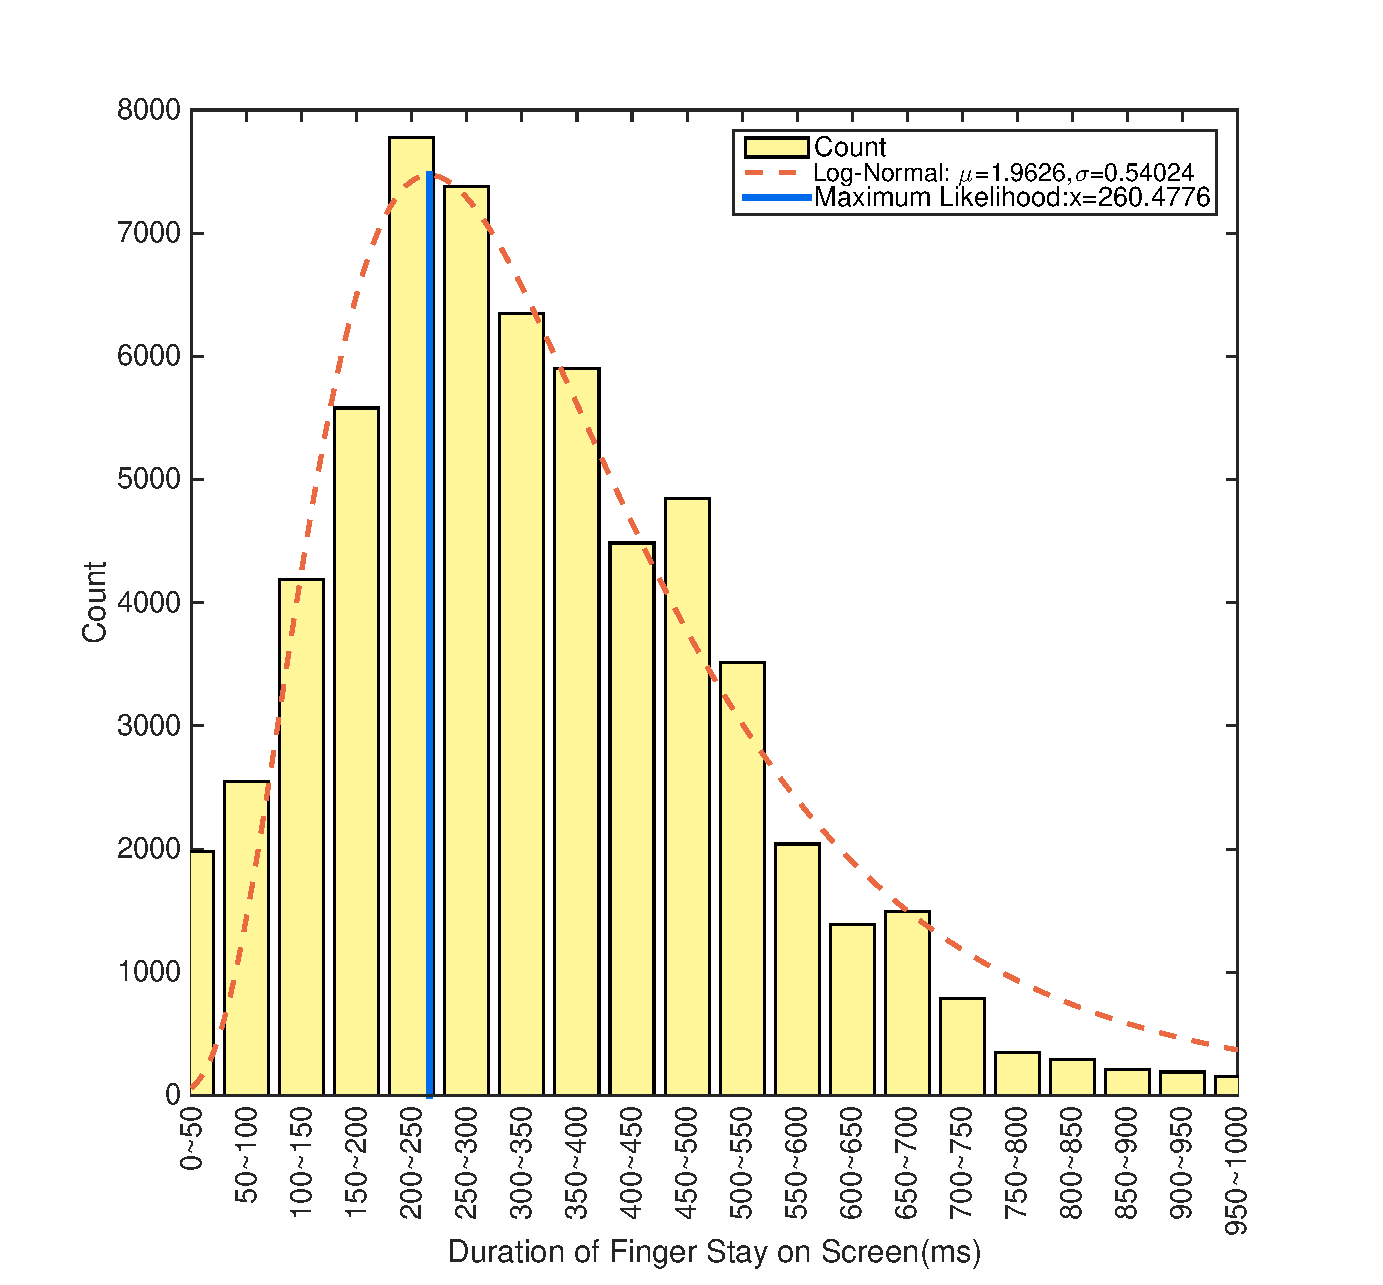
\includegraphics[width=0.5\textwidth]{figures/count-result}
    \caption{\kaishu 统计结果}
    \label{fig:result}
\end{figure}

从图\ref{fig:result} 的分布上我们可以看出,手指在屏幕上的停留时间主要集中在 260 ms 前后,呈对数正态分布。
对此,我们不妨将手指在屏幕上的平均停留时间设为 250 ms,故 DELAY 的值为 250ms;
另外,设 Force Touch 总持续时间为普通触摸事件的五倍,故 DURATION 的值为 1000ms;
这时触发 Force Touch 操作所需要的总时间为 1.25 秒。
对 Force Touch 而言,考虑人类手指的按压力度变化,我们设其力度的变化率线性变化,
这时能保证整条力度变化曲线为光滑曲线。

综上所述,记在一次按压中的按压时间为 $t_{\text{press}}$,
则 Force Touch 可以使用公式\ref{formal:delay}进行模拟:
\begin{equation}
v_{F} =
    \begin{cases}
        0    & \mbox{if $t_{\text{press}} < \text{DELAY}$} \\
        \left(\frac{t_{\text{press}}-\text{DELAY}}{\text{DURATION}}\right)^{2}
             & \mbox{if 0 < $t_{\text{press}}-\text{DELAY} < \text{DURATION}$} \\
        1    & \mbox{Otherwise}
    \end{cases}
\label{formal:delay}
\end{equation}
其中,$v_{F}$表示模拟的压力值,DELAY = 250,DURATION = 1000,两者单位为毫秒(ms),图像如图\ref{fig:ft-fig}所示。

\begin{figure}[htbp]
\centering
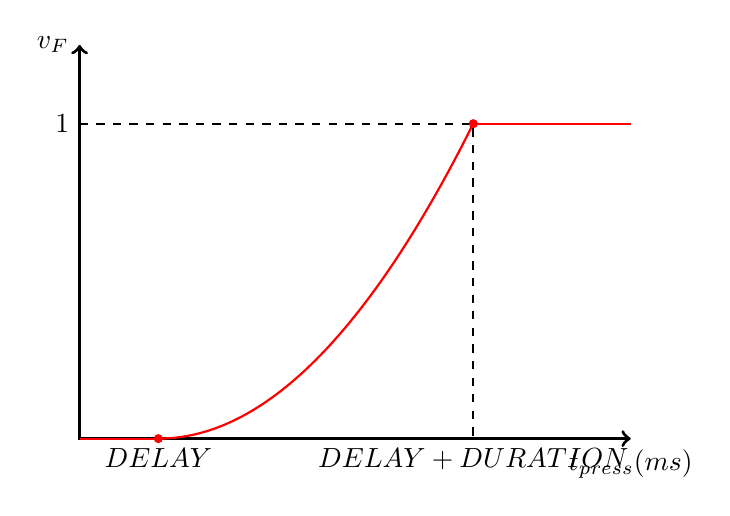
\begin{tikzpicture}[domain = 0:5, xscale = 1, yscale = 1]
    \draw [very thick, <->] (0, 5) node [left] {$v_{F}$}
             -- (0, 0) -- (7.0, 0) node [below] {$t_{\text{press}}\text{(ms)}$};

    \draw[domain=0:1, thick, smooth, color=red] plot(\x, 0);
    \draw[domain=1:5, thick, smooth, color=red] plot(\x, {0.25*(\x-1)^2});
    \draw[domain=5:7, thick, smooth, color=red] plot(\x, 4);

    \node[below] at (1.0, 0.0) {$\text{\tiny DELAY}$};

    \draw[thick, dashed] (0, 4) node [left] {1}
           -- (5,4) -- (5,0) node [below] {$\text{\tiny DELAY+DURATION}$};

    \draw[fill,color=red] (1,0) circle [radius=0.05];
    \draw[fill,color=red] (5,4) circle [radius=0.05];
\end{tikzpicture}
\caption{Force Touch 仿真函数的图像}
\label{fig:ft-fig}

\end{figure}

\subsection{Haptic Feedback Design}
在 watchOS 中\footnote{本文写成时的 watchOS 版本为 2.2。},
根据开发文档\cite{WatchGuide:2016}显示Haptic Engine 一共能表达代码\ref{lst:haptic-define}所示的几种类型。

\begin{lstlisting}[
    language={Swift},
    caption={\kaishu Haptic 反馈类型},
    label={lst:haptic-define}
]
public enum WKHapticType : Int {
    case Notification
    case DirectionUp
    case DirectionDown
    case Success
    case Failure
    case Retry
    case Start
    case Stop
    case Click
}
\end{lstlisting}

Success、Failure、Retry 三个 Haptic 类型均为对原生交互的操作执行结果的反馈,
于是我们将 Success 设置为备择交互中执行完操作且成功后的反馈,Failure 则对应为失败。
在原生交互时,Retry 只用于在输入密码时失败后的特殊情况,
不妨将此种情况的反馈依然用 Failure 表示,先保留此反馈类型,以便用于其他交互。

Notification 用于在休眠状态下的通知提醒,不对其进行修改;
DirectionUp 和 DirectionDown 是原生交互中 Digital Crown 旋转到顶端和底端时的反馈提醒,
对此我们同样继承此反馈设计,并扩展到数值调节中,当调整到数值最大值时,执行 DirectionUp 反馈,
反之执行 DirectionDown 反馈。

Start、Stop、Click 和 Retry 四个反馈类型恰好可以对拇指与食指、中指、
无名指捏合点击与 Force Touch 的四个个不同操作进行对应,
即 Click 表示普通点击事件,Stop 表示 ForceTouch 操作,
Start表示切换到下一视图,Retry 恰好用于切换到上一视图的提示反馈。

\section{The Interaction Completeless}
\label{sec:completeless}

\begin{figure}[H]
    \kaishu
    \centering
    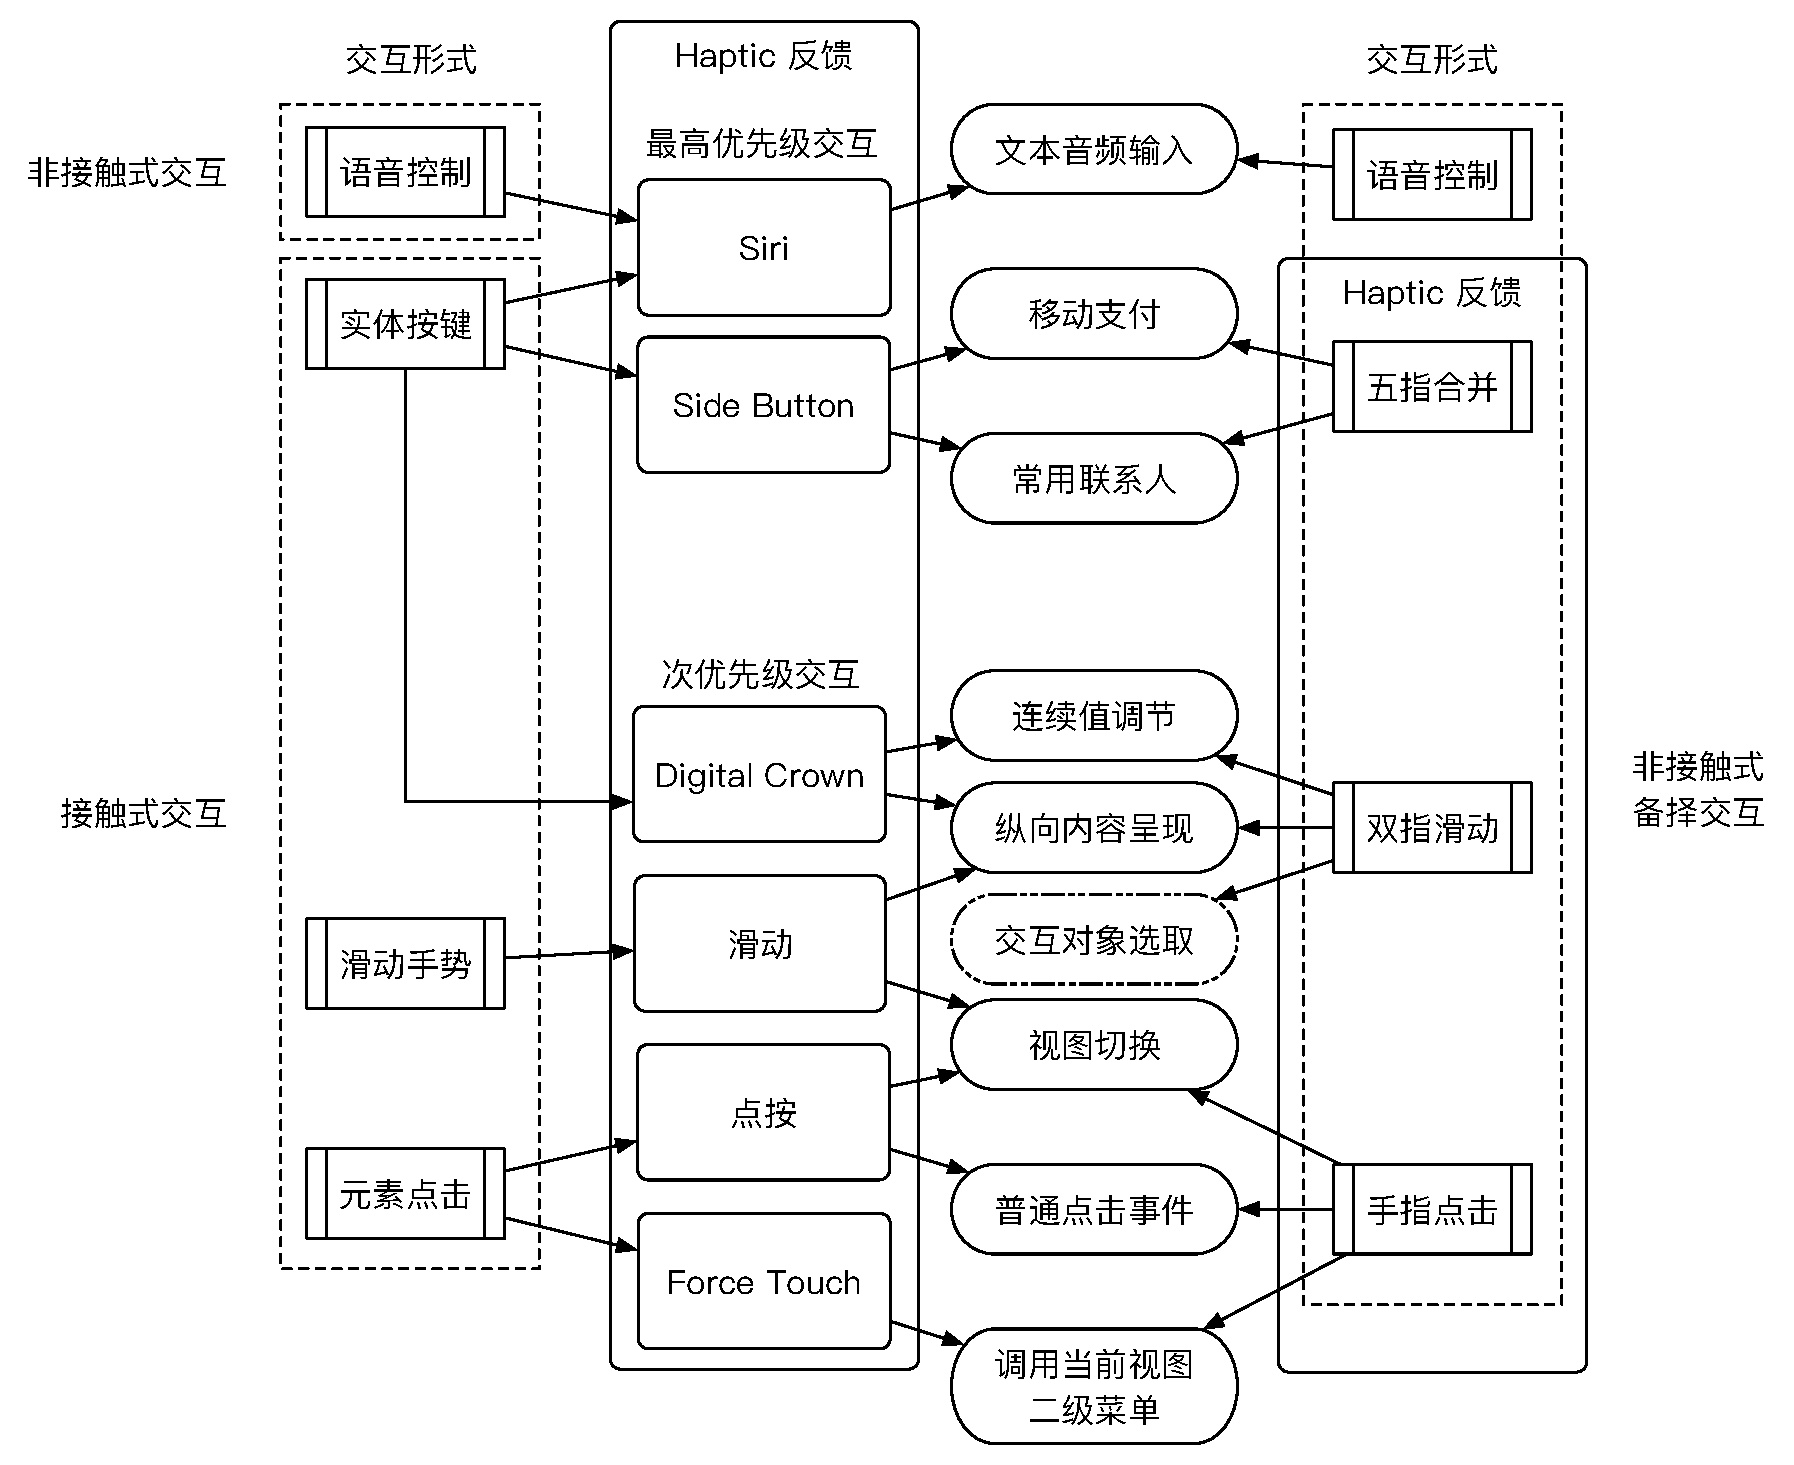
\includegraphics[width=0.5\textwidth]{figures/interaction}
    \caption{\kaishu 非接触式备择设计总览}
    \label{fig:interaction}
\end{figure}

本章中我们全面地对 Apple Watch 上的交互进行了重新设计,
简化了元素与元素之间的交互逻辑,作为小结,如图\ref{fig:interaction}。
在此套备择设计中,我们将原有的两层交互逻辑中十种不同交互逻辑通过简化为单层交互逻辑的八种,
并且消除了接触式交互这一限制。

从图\ref{fig:interaction}中我们容易看出,备择设计在交互上是完备的,即从另一个角度实现了原交互的全部功能。
